
\documentclass[11pt,notitlepage]{report}
\textwidth 15cm 
\textheight 21.3cm
\evensidemargin 6mm
\oddsidemargin 6mm
\topmargin -1.1cm
\setlength{\parskip}{1.5ex}

\usepackage{titlesec}
    \titleformat{\chapter}{\Large\centering}{}{0pt}{}{}

\usepackage{amsfonts,amsmath,amssymb,enumerate, amsthm, enumitem, stmaryrd, graphicx}  
\usepackage{enumitem}  
\usepackage{hyperref}
\usepackage{tikz}
\usepackage{hyperref, multicol}
\counterwithout{section}{chapter}
\newcommand{\bb}[1]{\ensuremath{\mathbb{#1}}}
\newcommand{\mc}[1]{\ensuremath{\mathcal{#1}}}
\newcommand{\mr}[1]{\ensuremath{\mathrm{#1}}}
\newcommand{\llp}[0]{\ensuremath{\llparenthesis}}
\newcommand{\rrp}[0]{\ensuremath{\rrparenthesis}}
\newcommand{\tbf}[1]{\textbf{#1}}
\newcommand{\modelsm}{\mathrel{\models\!\rvert}}
\newcommand{\vdashv}{\mathrel{\vdash\!\rvert}}
\newcommand\sbullet[1][.75]{\mathbin{\vcenter{\hbox{\scalebox{#1}{$\bullet$}}}}}

\makeatletter
\newcommand*{\toccontents}{\@starttoc{toc}}
\makeatother


\begin{document}
\parindent=0pt

\title{\vspace{-15mm}CS 245 Personal Notes \vspace{-5mm}}
\author{by Sam Gunter}
\date{Instructors: Jonathan Buss, Collin Roberts\\ 
Textbook: Mathematical Logic for Computer Science by Zhongwan Lu\\
Course Notes by: Collin Roberts\\
$\sbullet$ Spring 2021 $\sbullet$ University of Waterloo $\sbullet$}
\maketitle

\toccontents

\thispagestyle{empty}
\newpage
\setcounter{page}{1}
\tbf{Natural Deduction}
\vspace{-2mm}
\begin{enumerate}
    \item Reflexivity: $\rm A \vdash \rm A$ is a theorem
    \item $(+)$: If $\Sigma \vdash \rm A$, then $\Sigma, \Sigma' \vdash \rm A$ is a theorem
    \item $(\neg -)$: If $\Sigma, \neg \rm A \vdash \rm B$ and $\Sigma, \neg \rm A \vdash \neg \rm B$, then $\Sigma \vdash \rm A$ is a theorem
    \item $(\to -)$: If $\Sigma \vdash \rm A \to \rm B$ and $\Sigma \vdash \rm A$, then $\Sigma \vdash \rm B$ is a theorem
    \item $(\to +)$: If $\Sigma, \rm A \vdash \rm B$, then $\Sigma \vdash \rm A \to \rm B$ is a theorem
    \item $(\wedge -)$: If $\Sigma \vdash \rm A \wedge \rm B$, then $\Sigma \vdash \rm A$ and $\Sigma \vdash \rm B$ are theorems
    \item $(\wedge +)$: If $\Sigma \vdash \rm A$ and $\Sigma \vdash \rm B$, then $\Sigma \vdash \rm A \wedge \rm B$ is a theorem
    \item $(\vee -)$: If $\Sigma, \rm A \vdash \rm C$ and $\Sigma, \rm B \vdash \rm C$, then $\Sigma, \rm A \vee \rm B \vdash \rm C$ is a theorem
    \item $(\vee +)$: If $\Sigma \vdash \rm A$, then $\Sigma \vdash \rm A \vee \rm B$ and $\Sigma \vdash \rm B \vee A$ are theorems
    \item $(\leftrightarrow -)$: If $\Sigma \vdash \rm A \leftrightarrow \rm B$ and $\Sigma \vdash \rm B$, then $\Sigma \vdash \rm A$ is a theorem
    \item $(\leftrightarrow + )$: If $\Sigma, \rm A \vdash \rm B$ and $\Sigma, \rm B \vdash \rm A$, then $\Sigma \vdash \rm A \leftrightarrow \rm B$ is a theorem
    \item $(\forall -)$: If $\Sigma \vdash \rm \forall x A(x)$, then for a term $\rm t$, $\Sigma \vdash \rm A(t)$ is a theorem
    \item $(\forall +)$: If $\Sigma \vdash \rm A(u)$ and $\rm u \not \in \Sigma$, then $\rm \Sigma \vdash \forall x \rm A(x)$ is a theorem
    \item $(\exists -)$: If $\rm \Sigma, A(u) \vdash B$ and $\rm u \not \in \Sigma \cup \rm B$, then $\rm \Sigma, \exists x A(x) \vdash B$ is a theorem
    \item $(\exists +)$: If $\rm \Sigma \vdash A(t)$, then for $\rm A'(x)$ such that some occurrences of $\rm t$ in $\rm A(t)$ are replaced by $\rm x$, $\rm \Sigma \vdash \exists x \rm A'(x)$ is a theorem
    \item $(\approx -)$: If $\rm \Sigma \vdash A(t_1)$ and $\rm \Sigma \vdash t_1 \approx t_2$, then for $\rm A'(t_2)$ such that some occurrences of $\rm t_1$ in $\rm A(t_1)$ are replaced by $\rm t_2$, $\rm \Sigma \vdash A'(t_2)$ is a theorem
    \item $(\approx +)$: $\emptyset \rm \vDash u \approx u$ is a theorem
    \item Membership Rule $(\in)$: If $\rm A \in \Sigma$, then $\Sigma \vdash \rm A$
\end{enumerate}
\tbf{Peano's Axioms}
\vspace{-2mm}
\begin{enumerate}[label=PA\arabic*:]
    \item $\forall \rm x(s(x) \not \approx 0)$
    \item $\forall \rm x \forall y ((s(x) \approx s(y)) \to (x \approx y))$
    \item $\forall \rm x(x + 0 \approx x)$
    \item $\forall \rm x \forall y ((x + s(y)) \approx s(x+y))$
    \item $\forall \rm x(s(x) \cdot 0 = 0)$
    \item $\forall \rm x \forall y (x \cdot s(y) = x \cdot y + x)$
    \item Axiom Schema: For a formula $\rm A(u)$ where $\rm u$ is a free variable,
    $$\rm (A(0) \wedge \forall x(A(x) \to A(s(x)))) \to \forall x A(x)$$
\end{enumerate}
\newpage



\newpage

\section{Introduction}

\textbf{Def} Logic: From the Greek word Logykos, reasoning. The science of proof, the fundamental science of thought, the art of applying knowledge, the analysis of arguments

\begin{itemize}
    \item Plato (429-327BC) studies ``What is Truth"
    \item Aristotle (384-322BC) lays down the first systemic treatment of valid reasoning ``syllogisms"
    \item Rene Descartes (1596-1650) introduces algebraic symbols into geometry
    \item George Boole (1815-1864) proposes the use of algebra for logic
    \item Kurt Goel (1906-1978) demonstrates that any theory must have limitations
    \item Alan Turing (1912-1954) gives the first definition of computer prorgamming
\end{itemize}

\textbf{Def} Syllogism: A kind of logical argument where a proposition is inferred from two others (premises) \\
\hspace*{5mm} Note: Based on form, not content

\textbf{Applications:}
\begin{enumerate}
    \item Electronic digital circuits formed from logic gates to minimize components
    \item Artificial Intelligence uses knowledge base and an inference engine
    \begin{enumerate}
        \item DENDRAL to identify unknown organic molecules
        \item MYCIN to treat blood infections to the same degree as a specialist in blood infections
        \item MISTRAL to monitor dam safety
    \end{enumerate}
    \item Automated Proof Verifiers
    \item Databases such as SQL use first order logic
    \item Software Design/Programming Languages
    \item DNA Computing
    \item Synthetic Biology
\end{enumerate}
\newpage

\textbf{Def} Truth-Preserving: If the premises are true, then the conclusion must be true

\textbf{Def} Logic: The analysis and appraisal of arguments

\textbf{Def} Argument: A set of statements including premise(s) and a conclusion

\textbf{Def} Valid: An argument is valid, correct, or sound when if its premises are true its conclusion is true

\textbf{Def} Compound Statements: Consists of several parts, each of which is its own statement

\textbf{Def} Hypothetical Syllogism: If $\rm p$ then $\rm q$, if $\rm q$ then $\rm r$, therefore if $\rm p$ then $\rm r$

\textbf{Def} Disjunctive Syllogism: $\rm p$ or $\rm q$, not $\rm q$, therefore $\rm p$

\textbf{Def} Modus Ponens: If $\rm p$ then $\rm q$, $\rm p$, therefore $\rm q$

\textbf{Def} Proposition: A statement with a true or false value\\
\hspace*{5mm} Variable: any variable ($\rm p, \rm q, \rm r$)\\
\hspace*{5mm} Constants: 1 or true and 0 or false

\textbf{Def} Atomic Propositions: Cannot be further divided, a single variable

\tbf{Def} Compound Propositions: Combination of several variables

\tbf{Def} Logical Connectives: or, and, not, if, then, equivalence\\
\hspace*{5mm} Unary Connective: not or negation\\
\hspace*{5mm} Binary Connective: or, and, if, then, equivalence\\
\hspace*{5mm} Symmetric: or, and, equivalence

\tbf{Def} Negation: Not ``reverses" the truth value of the proposition
$$\neg \rm p$$

\tbf{Def} Conjunction: True if both are true, false otherwise
$$\rm p \wedge \rm q$$

\tbf{Def} Disjunction: False if both are false, true otherwise
$$\rm p \vee \rm q$$

\tbf{Def} Implication: If a proposition (antecedent) implies another (consequent)
$$\rm p \to \rm q$$
\hspace*{5mm} Vacuously True: If $\rm p \to \rm q$ but $\rm \neg p$, then always true

\tbf{Def} Equivalence: Or biconditional, a double implication
$$\rm p \leftrightarrow \rm q$$

\section{Propositional Language: Syntax}

\tbf{Def} Propositional Language $\mc L^p$: The formal language of propositional logic which is expressions from a set of symbols
\begin{itemize}
    \item Proposition Symbols: $\mathrm p, \rm q, \rm r, \dots$
    \item Connective Symbols: $\neg, \vee, \wedge, \to, \leftrightarrow$
    \item Punctuation Symbols: $(, )$
\end{itemize}

\tbf{Def} Expressions: Finite strings of the allowed symbols where the length is the number of occurrences of symbols, often defined by $\mathrm U, \mathrm V, etc$ (Meta-symbols, along with $=, \ne$)\\
\hspace*{5mm} Empty Expression: $\varepsilon$

\tbf{Def} Concatenation: An expression followed by another expression $UV$\\
\hspace*{5mm} Note: $\rm U\varepsilon = \rm U$

\tbf{Def} Segment: If $\rm U = \rm W_1 \rm V \rm W_2$ then $\rm V$ is a segment of $\rm U$\\
\hspace*{5mm} if $\rm V \ne \rm U$, then a Proper Segment\\
\hspace*{5mm} if $\rm U = \rm V \rm W$, then $\rm V$ is an Initial Segment\\
\hspace*{5mm} if $\rm U = \rm W\rm V$, then $\rm V$ is a Terminal Segment

\tbf{Def} Atomic Formula: An expression with length 1 consisting of a variable
$$Atom(\mc L^p)$$

\tbf{Def} Formulas: The set $Form(\mathcal L^p)$ that meet the formation rules
\begin{itemize}
    \item Every $Atom(\mc L^p)$ is in $Form(\mc L^p)$
    \item For $\rm A, \rm B \in Form(\mc L^p)$
    \begin{itemize}
        \item $(\neg \rm A) \in Form(\mc L^p)$
        \item $(\rm A \wedge \rm B) \in Form(\mc L^p)$
        \item $(\rm A \vee \rm B) \in Form(\mc L^p)$
        \item $(\rm A \to \rm B) \in Form(\mc L^p)$
        \item $(\rm A \leftrightarrow \rm B) \in Form(\mc L^p)$
    \end{itemize}
\end{itemize}

\tbf{Theorem} Unique Readability: Every formula of $Form(\mc L^p)$ is of exactly one of the six forms in exactly one way

\tbf{Lemma} Every Formula in $Form(\mc L^p)$ has an equal number of left and right parentheses

\tbf{Theorem} Every Formula in $Form(\mc L^p)$ is an atom or one of the six forms

\newpage
\tbf{Def} Precedence Rules: To aid in removing brackets, the connective symbols should be read in order of
\begin{itemize}
    \item $\neg$
    \item $\wedge$
    \item $\vee$
    \item $\to$
    \item $\leftrightarrow$
\end{itemize}

\tbf{Def} Scopes: For $(\neg \rm A)$, $\rm A$ is the scope of this negation. For $(\rm A *' \rm B)$, $\rm A$ is the left scope and $\rm B$ is the right scope


\section{Propositional Language: Semantics}

\textbf{Def} Semantics: The meaning of logic (where syntax is the formation)

\textbf{Def} Truth Value: A function that maps to true or false, $\{0, 1\}$
$$t: Atom(\mc L^p) \mapsto \{0, 1\}$$

\textbf{Def} Truth Table: Lists all possible truth valuations\\
\hspace*{5mm} Truth valuation: A single row

\textbf{Def} Value: The value of $A$ with respect to $t$ is
$$A^t = \begin{cases}\text{if }Atom(A), &t(p)\\
\text{if } A = (\neg B)^t, &\begin{cases}1 & \text{if }B^t = 0\\0 & \text{if }B^t = 1\end{cases}\\
\text{if } A = (B \wedge C)^t, &\begin{cases}1 & \text{if }B^t = C^t = 1\\0 & \text{else}\end{cases}\\
\text{if } A = (B \vee C)^t, &\begin{cases}1 & \text{if }B^t \ne 0 \ne C^t\\0 & \text{else}\end{cases}\\
\text{if } A = (B \to C)^t, &\begin{cases}1 & \text{if }B^t = 0 \text{ or } C^t = 1\\0 & \text{else}\end{cases}\\
\text{if } A = (B \leftrightarrow C)^t, &\begin{cases}1 & \text{if }B^t = C^t\\0 & \text{else}\end{cases}\\
\end{cases}$$


\textbf{Def} Satisfiable: For given formulas $\Sigma \in Form(\mc L^p)$, if and only if there exists a $t$ such that for all formulas $\Sigma^t = 1$ is satisfied ($\Sigma^t = 0$ if at least 1 formula does not satisfy)\\
\hspace*{5mm} Note: $t$ satisfies, $\Sigma$ is satisfied

\textbf{Def} Tautology: A formula which is true under all truth valuations
$$A^t = 1, \forall t$$

\textbf{Def} Contradiction: A formula which is false under all truth valuations
$$A^t = 0, \forall t$$

\textbf{Def} Contingent: A formula which may be true or false depending on truth valuation

\textbf{Def} Law of the Excluded Middle: $\rm p \vee \neg \rm p$ is a tautology

\textbf{Theorem} Let $A$ be a tautology with proposition symbols $\rm p_1, \rm p_2, \dots \rm p_n$, then replacing $\rm p_i$ with arbitrary formula $B$ is also a tautology

\textbf{Def} Law of the Contradiction: $\rm p \wedge \neg \rm p$ is a contradiction

\textbf{Def} Law of identity: The final of Plato's essential thoughts, $\rm p = \rm p$

\textbf{Def} Tautological Consequence: For $\Sigma, A \in Form(\mc L^p)$, $\Sigma$ tautologically entails $A$ if and only if
$$\Sigma \vDash A: \forall t, \Sigma^t = 1 \to A^t = 1$$
\hspace*{5mm} $\emptyset \vDash A$ is true for all $A \in Form(\mc L^p)$ is $A$ is a tautology

\textbf{Def} Valid:
\begin{itemize}
    \item The argument with premises $A_1, A_2, \dots A_n$ and conclusion $C$ is valid
    \item $(A_1 \wedge A_2 \wedge \dots \wedge A_n) \to C$ is a tautology
    \item $(A_1 \wedge A_2 \wedge \dots \wedge A_n \wedge \neg C)$ is a contradiction
    \item $(A_1 \wedge A_2 \wedge \dots \wedge A_n \wedge \neg C)$ is not satisfiable
    \item $\{A_1, A_2, \dots A_n, \neg C\}$ is not satisfiable
    \item $\{A_1, A_2, \dots A_n\} \vDash C$
\end{itemize}

\textbf{Def} Tautologically Equivalent: If $A \vDash B$ and $B \vDash A$ then
$$A \modelsm B$$
\hspace*{5mm} Note: Equality implies equivalence but not vice versa

\textbf{Def} Proof by Contradiction: Assume the contrary, reach a contradiction

\textbf{Def} De Morgan's Law: 
$$\neg(\rm p \wedge \rm q) \modelsm (\neg \rm p \vee \neg \rm q)$$

\textbf{Def} Dual De Morgan's Law: 
$$\neg(\rm p \vee \rm q) \modelsm (\neg \rm p \wedge \neg \rm q)$$

\textbf{Def} Contrapositives: 
$$(\rm p \to \rm q) \modelsm (\neg \rm q \to \neg \rm p)$$

\textbf{Def} Bi-Conditional: 
$$\rm p \leftrightarrow \rm q \modelsm (\rm p \to \rm q) \wedge (\rm q \to \rm p)$$

\textbf{Lemma} Tautological Equivalences: Let $A \modelsm A'$ and $B \modelsm B'$, then
\begin{enumerate}
    \item $\neg A \modelsm \neg A'$
    \item $A \wedge B \modelsm A' \wedge B'$
    \item $A \vee B \modelsm A' \vee B'$
    \item $A \to B \modelsm A' \to B'$
    \item $A \leftrightarrow B \modelsm A' \leftrightarrow B'$
\end{enumerate}

\tbf{Theorem} Replaceability of Tautologically Equivalent Formulas: Let $B \modelsm B'$, and $A'$ be $A$ with some instances of $B$ replaced by $B'$, then $A' \modelsm A$

\tbf{Theorem} Duality: Let $A$ be composed of atoms, $\neg, \wedge, \vee$, then for $\Delta(A)$ made by replacing all atoms with their negation and all $\vee$ with $\wedge$ (and vice versa), $\neg A \modelsm \Delta(A)$

\tbf{Def} Fuzzy Logic: Uses real values within $[0, 1]$ to denote partial truth where the restriction to $\{0, 1\}$ coincides with classical logic, now 
\begin{itemize}
    \item And$(x, y) = \min\{x, y\}$
    \item Or$(x, y) = \max\{x, y\}$
    \item Not$(x) = 1 - x$
\end{itemize}
\vspace{-2mm}

\section{Propositional Calculus: Essential Laws, Normal Forms}

\textbf{Def} Tautological Equivalences: 
\vspace{-2mm}
\begin{itemize}
    \item $(A \wedge B) \wedge C \modelsm A \wedge (B \wedge C)$
    \item $1 \wedge \neg A \modelsm 0$
    \item $1 \wedge 0 \modelsm 0$
\end{itemize}

\textbf{Def} Removing the Connectives: Connectives are definable (or reducible) in terms of $\neg, \wedge, \vee$
\vspace{-2mm}
\begin{itemize}
    \item $A \to B \modelsm \neg A \vee B$
    \item $A \leftrightarrow B \modelsm (A \wedge B) \vee (\neg A \wedge \neg B) \modelsm (\neg A \vee B) \wedge (\neg B \vee A)$
\end{itemize}

\newpage
\tbf{Propositional Calculus Laws} By dual pairs,
\begin{itemize}
    \item Excluded Middle Law: $A \vee \neg A \modelsm 1$
    \item Contradiction Law: $A \wedge \neg A \modelsm 0$
    \item Identity Laws: $A \vee 0 \modelsm A$, $A \wedge 1 \modelsm A$
    \item Domination Laws: $A \vee 1 \modelsm 1$, $A \wedge 0 \modelsm 0$
    \item Idempotent Laws: $A \vee A \modelsm A$, $A \wedge A \modelsm A$
    \item Double-Negation Laws: $\neg (\neg A)\modelsm A$
    \item Conductivity Laws: $A \vee B \modelsm B \vee A$, $A \wedge B \modelsm B \wedge A$
    \item Associativity Laws: $(A \vee B) \vee C \modelsm A \vee (B \vee C)$, $(A \wedge B) \wedge C \modelsm A \wedge (B \wedge C)$
    \item Distributivity Laws: $A \vee (B \wedge C) \modelsm (A \vee B) \wedge (A \vee C)$, $A \wedge (B \vee C) \modelsm (A \wedge B) \vee (A \wedge C)$
    \item De Morgan's Laws: $\neg(A \wedge B) \modelsm \neg A \vee \neg B$, $\neg(A \vee B) \modelsm \neg A \wedge \neg B$
    \item Absorption Laws: $A \vee (A \wedge B) \modelsm A$, $A \wedge (A \vee B) \modelsm A$
    \item Another Important Law (lec 4, pg 9): $(A \wedge B) \vee (\neg A \wedge B) \modelsm B$, $(A \vee V) \wedge (\neg A \vee B) \modelsm B$
\end{itemize}

\textbf{Def} Literal: Complementary literals are of the form $\rm p, \neg \rm p$ 

\textbf{Def} Disjunctive Clause: A disjunction with literals as disjuncts 
$$(\rm p \vee \neg \rm q \vee \rm s)$$

\textbf{Def} Conjunctive Clause: A conjunction with literals as conjuncts
$$(\rm p \wedge \neg \rm q \wedge \rm s)$$

\textbf{Def} Disjunctive Normal Form: A disjunction with conjunctive clauses
$$\rm p \vee (\rm q \wedge \rm r)$$

\textbf{Def} Conjunctive Normal Form: A conjunction with disjunctive clauses
$$\rm p \wedge (\rm q \vee \rm r) \wedge (\neg \rm q \vee \rm r)$$

\textbf{Theorem (lec 4 pg 23)} Any formula $A \in Form(\mc L^p)$ is tautologically equivalent to some formula in disjunctive normal form

\textbf{Theorem (lec 4 pg 24)} Any formula $A \in Form(\mc L^p)$ is tautologically equivalent to some formula in conjunctive normal form


\section{Adequate Set of Connectives}

\textbf{Def} $n-$ary Connectives: A connective $f(\rm A_1, \rm A_2, \dots \rm A_n)$ is defined by its truth-table\\
\hspace*{5mm} Note: There are 4 distinct unary connectives\\
\hspace*{5mm} Note: There are 16 distinct binary connectives

\begin{center}
\begin{tabular}{ |c|c || c|c|c|c|c|c|c|c|c|c|c|c|c|c|c|c| } 
 \hline
 $\rm p$ & $\rm q$ & $\top$ & $\vee$ & $\leftarrow$ & $\to$ & $\mid$ & $\rm p$ & $\rm q$ & XOR & $\leftrightarrow$ & $\neg \rm q$ & $\neg \rm p$ & $\wedge$ & $f$ & $f$ & $\downarrow$ & $\bot$ \\ 
 \hline
 1 & 1 & 1 & 1 & 1 & 1 & 0 & 1 & 1 & 0 & 1 & 0 & 0 & 1 & 0 & 0 & 0 & 0 \\ 
 1 & 0 & 1 & 1 & 1 & 0 & 1 & 1 & 0 & 1 & 0 & 1 & 0 & 0 & 1 & 0 & 0 & 0 \\ 
 0 & 1 & 1 & 1 & 0 & 1 & 1 & 0 & 1 & 1 & 0 & 0 & 1 & 0 & 0 & 1 & 0 & 0 \\ 
 0 & 0 & 1 & 0 & 1 & 1 & 1 & 0 & 0 & 0 & 1 & 1 & 1 & 0 & 0 & 0 & 1 & 0 \\ 
 \hline
\end{tabular}
\end{center}

\textbf{Def} Adequate: A set of connectives is adequate if they can express every truth table\\
\hspace*{5mm} Note: The standard connectives are adequate $\{\neg, \wedge, \vee, \to, \leftrightarrow\}$

\tbf{Theorem (Logic 5, pg 8)}: The set $\{\neg, \wedge, \vee\}$ is adequate

\tbf{Corollary (Logic 5, pg 10)}: The sets $\{\neg, \wedge\}, \{\neg, \vee\}$, $\{\neg, \to\}$ are adequate

\textbf{Def} NOR: The Peirce arrow connective
\begin{center}
\begin{tabular}{ |c|c || c| } 
 \hline
 $\rm p$ & $\rm q$ & $\rm p \downarrow \rm q$ \\ 
 \hline
 1 & 1 & 0 \\ 
 1 & 0 & 0 \\ 
 0 & 1 & 0 \\ 
 0 & 0 & 1 \\ 
 \hline
\end{tabular}
\end{center}

\textbf{Def} NAND: The Sheffer stroke connective
\begin{center}
\begin{tabular}{ |c|c || c| } 
 \hline
 $\rm p$ & $\rm q$ & $\rm p \mid \rm q$ \\ 
 \hline
 1 & 1 & 0 \\ 
 1 & 0 & 1 \\ 
 0 & 1 & 1 \\ 
 0 & 0 & 1 \\ 
 \hline
\end{tabular}
\end{center}

\textbf{Def} Ternary Connective: The if, then, else connective
\begin{center}
\begin{tabular}{ |c|c|c || c| } 
 \hline
 $\rm p$ & $\rm q$ & $\rm r$ & $\tau(\rm p, \rm q, r)$ \\ 
 \hline
 1 & 1 & 1 & 1\\ 
 1 & 1 & 0 & 1\\ 
 1 & 0 & 1 & 0\\ 
 1 & 0 & 0 & 0\\ 
 0 & 1 & 1 & 1\\ 
 0 & 1 & 0 & 0\\ 
 0 & 0 & 1 & 1\\ 
 0 & 0 & 0 & 0\\ 
 \hline
\end{tabular}
\end{center}

\section{Propositional Logic: Formal Deduction}


\textbf{Def} Formal Deduction: A relation between a set of premises and conclusion formulas
$$\{\rm A_1, \rm A_2, \dots\} = \Sigma \vdash \rm A \text{ where }\Sigma \cup \rm A = \Sigma, \rm A$$

\textbf{Def} Proof: A finite sequence of sequents ($\Sigma_i \vdash \rm A_i$)\\
\hspace*{5mm} Note: A Theorem is the final sequent in a valid proof

\textbf{Def} Natural Deduction: A set of eleven rules (or schema)
\begin{enumerate}
    \item Reflexivity: $\rm A \vdash \rm A$ is a theorem
    \item Addition of Premises: If $\Sigma \vdash \rm A$, then $\Sigma, \Sigma' \vdash \rm A$ is a theorem
    \item $\neg$ Elimination: If $\Sigma, \neg \rm A \vdash \rm B$ and $\Sigma, \neg \rm A \vdash \neg \rm B$, then $\Sigma \vdash \rm A$ is a theorem
    \item $\to$ Elimination: If $\Sigma \vdash \rm A \to \rm B$ and $\Sigma \vdash \rm A$, then $\Sigma \vdash \rm B$ is a theorem
    \item $\to$ Introduction: If $\Sigma, \rm A \vdash \rm B$, then $\Sigma \vdash \rm A \to \rm B$ is a theorem
    \item $\wedge$ Elimination: If $\Sigma \vdash \rm A \wedge \rm B$, then $\Sigma \vdash \rm A$ and $\Sigma \vdash \rm B$ are theorems
    \item $\wedge$ Introduction: If $\Sigma \vdash \rm A$ and $\Sigma \vdash \rm B$, then $\Sigma \vdash \rm A \wedge \rm B$ is a theorem
    \item $\vee$ Elimination: If $\Sigma, \rm A \vdash \rm C$ and $\Sigma, \rm B \vdash \rm C$, then $\Sigma, \rm A \vee \rm B \vdash \rm C$ is a theorem
    \item $\vee$ Introduction: If $\Sigma \vdash \rm A$, then $\Sigma \vdash \rm A \vee \rm B$ and $\Sigma \vdash \rm B \vee A$ are theorems
    \item $\leftrightarrow$ Elimination: If $\Sigma \vdash \rm A \leftrightarrow \rm B$ and $\Sigma \vdash \rm B$, then $\Sigma \vdash \rm A$ is a theorem
    \item $\leftrightarrow$ Introduction: If $\Sigma, \rm A \vdash \rm B$ and $\Sigma, \rm B \vdash \rm A$, then $\Sigma \vdash \rm A \leftrightarrow \rm B$ are theorems
    \item Membership Rule $\in$: If $\rm A \in \Sigma$, then $\Sigma \vdash \rm A$
\end{enumerate}

\textbf{Def} Formal Proof: Formula $\rm A$ is formally deducible from $\Sigma$ if and only if $\Sigma \vdash \rm A$ is generate by a finite applications of the rules of formal deduction

\tbf{Def} Semantics: Considers what is true or false
$$A \vDash B \text{ iff } A \to B \text{ is a tautology}$$

\tbf{Def} Syntax: Formulas are merely a sequence of abstract symbols
$$A \vdash B \text{ iff } \emptyset \vdash A \to B$$

\tbf{Lemma} Double-Negation Elimination $(\neg \neg -)$: For every $\rm A$,
$$\neg \neg \rm A \vdash \rm A$$

\tbf{Theorem} Reductio Ad Absurdum $(\neg +)$: If $\Sigma, \rm A \vdash \rm B$ and $\Sigma, \rm A \vdash \neg \rm B$, then 
$$\Sigma \vdash \neg \rm A$$

\tbf{Lemma} Contrapositive: For every $\rm A, \rm B$,
$$\rm A \to \rm B \vdash \neg \rm B \to \neg \rm A$$

\tbf{Theorem} Transitivity of Deducibility (Tr): Let $\Sigma \subseteq Form(\mc L^p)$, $\rm A_1, \rm A_2, \dots \rm A_n \in Form(\mc L^p)$. If $\Sigma \vdash \rm A_i$ for all $i \in \{1,2,\dots n\}$ and $\rm A_1, \rm A_2, \dots \rm A_n \vdash \rm A$, then
$$\Sigma \vdash \rm A$$

\tbf{Def} Syntactically Equivalent: When $A \vdashv B$ holds

\tbf{Lemma} Syntactic Equivalence: If $\rm A \vdashv A'$ and $\rm B \vdashv B'$, then
\begin{enumerate}[label=\roman*)]
    \item $\neg \rm A \vdashv \neg \rm A'$
    \item $\rm A \wedge \rm B \vdashv \rm A' \wedge \rm B'$
    \item $\rm A \vee \rm B \vdashv \rm A' \vee \rm B'$
    \item $\rm A \to \rm B \vdashv \rm A' \to \rm B'$
    \item $\rm A \leftrightarrow \rm B \vdashv \rm A' \leftrightarrow \rm B'$
\end{enumerate}

\tbf{Theorem} Replacement of Syntactically Equivalent Formulas (Repl): Let $\rm B \vdashv \rm C$, for a given $\rm A$, Let $\rm A'$ be constructed from the replacement of some occurances of $\rm B$ with $\rm C$, then
$$\rm A \vdashv \rm A'$$

\tbf{Theorem} Finiteness of Premise Set: If $\Sigma \vdash \rm A$, then $\exists \Sigma_0 \subseteq \Sigma$ such that $\Sigma_0 \vdash \rm A$

\tbf{Def} Soundness: Every statement that one proves should be actually correct

\tbf{Def} Completeness: One should be able to prove, within the system, every correct statement

\tbf{Theorem} Soundness and Completeness: Natural Deduction is both sound and complete for propositional logic, that is
$$\forall \Sigma, \rm A, \text{ if }\Sigma \vdash \rm A, \text{ then }\Sigma \vDash \rm A$$
$$\forall \Sigma, \rm A, \text{ if }\Sigma \vDash \rm A, \text{ then }\Sigma \vdash \rm A$$

\tbf{Fallacy} Denying the Antecedent: $\rm p \to \rm q, \neg \rm p \vdash \neg \rm q$

\tbf{Fallacy} Affirming the Consequent: $\rm p \to \rm q, \rm q \vdash \rm p$

\tbf{Def} Inconsistent: When there is a formula $\rm A$ such that for the set $\Sigma$, $\Sigma \vdash \rm A$ and $\Sigma \vdash \neg \rm A$

\tbf{Lemma} Inconsistent Sets: Let $\Sigma$ be a set of formulas, $\Sigma$ is inconsistent if and only if for every $\rm B$, $\Sigma \vdash \rm B$ 

\tbf{Def} Consistent: There is no formula $\rm A$ such that $\Sigma \vdash \rm A$ and $\Sigma \vdash \neg \rm A$

\tbf{Lemma} Consistent Sets: Let $\Sigma$ be a set of formulas, $\Sigma$ is consistent if and only if there exists a $\rm B$ such that $\Sigma \not \vdash \rm B$ 

\tbf{Lemma} Proof and Inconsistency: Let $\Sigma$ be a set of formulas, and $\rm A$ is a formula, then
$$\Sigma \vdash \rm A \text{ if and only if } \Sigma \cup \{\neg \rm A\} \text{ is inconsistent}$$
$$\Sigma \not \vdash \rm A \text{ if and only if } \Sigma \cup \{\neg \rm A\} \text{ is consistent}$$

\tbf{Lemma} Proof and Inconsistency Semantic Analogue: Let $\Sigma$ be a set of formulas, and $\rm A$ is a formula, then
$$\Sigma \vDash \rm A \text{ if and only if } \Sigma \cup \{\neg \rm A\} \text{ is unsatisfiable}$$
$$\Sigma \not \vDash \rm A \text{ if and only if } \Sigma \cup \{\neg \rm A\} \text{ is satisfiable}$$

\tbf{Def} Maximal: A consistent set such that for every formula $\rm A$, either $\rm A \in \Sigma$ or $\neg \rm A \in \Sigma$

\tbf{Lemma} Maximal Consistent Sets: Let $\Sigma$ be a maximal consistent set, then for every $\rm A$,
$$\Sigma \vdash \rm A \Longleftrightarrow \rm A \in \Sigma$$

\tbf{Theorem} Soundness of Propositional Formal Deduction: For all $\Sigma, \rm C$, if $\Sigma \vdash \rm C$, then $\Sigma \vDash \rm C$ 

\tbf{Theorem} Soundness of Propositional Formal Deduction 2: If $\Sigma$ is satisfiable, then $\Sigma$ is consistent

\tbf{Theorem} Completeness of Propositional Formal Deduction: For all $\Sigma, \rm A$, if $\Sigma \vDash \rm A$, then $\Sigma \vdash \rm A$ 

\tbf{Lemma} Maximal Consistent: Let $\rm M$ be a maximal consistent set $\rm M = \cup_{i=0}^\infty \Sigma_i$ for proposition formulas such that $\Sigma_{i+1} = \Sigma_i \cup \{\rm A_i\}$ if $\Sigma_i \cup \{\rm A_i\}$ is consistent
\begin{enumerate}[label=MC\arabic*:]
    \item For every $\rm A$, either $\rm A \in \rm M$ or $\neg \rm A \in \rm M$ but not both
    \item If $\rm M \vdash \rm A$, then $\rm A \in \rm M$
    \item For every $\rm A, \rm B$, if $\rm A \in \rm M$ and $\rm A \to \rm B \in \rm M$, then $\rm B \in \rm M$
    \item For every $\rm B \in \rm M$, for every $\rm A$, $\rm A \to \rm B \in \rm M$
    \item For every $\rm A \not\in \rm M$, for every $\rm B$, $\rm A \to \rm B \in \rm M$
\end{enumerate}

\newpage
\section{Propositional Logic: Resolution}

\tbf{Def} Resolution: A method to to prove a disjunctive clause by proving that $\{\rm A_1, A_2, \dots A_n, \neg C\}$ is not satisfiable (leads to  a contradiction) using the formal deduction rule with parents clauses $(\rm C \vee p, \rm D \vee \neg p)$ and the resolvent $(\rm C \vee D)$. Two clauses can be resolved if and only if they contain complementary literals $(\rm p, \neg \rm p)$ in which case they resolve over $\rm p$
$$\rm C \vee p, \rm D \vee \neg p \vdash_r C \vee D$$
\hspace*{5mm} Empty Clause: The resolvent of $\rm p, \neg p \vdash_r \{\}$

\tbf{Def} Resolution Derivation: From a set of clauses $\rm S$, the finite set of clauses such that each clause is in $\rm S$ or results from $\rm S$

\tbf{Def} Resolution Procedure: For $\rm S = \{\rm D_1, D_2, \dots D_m\}$, choose two clauses that contain $\rm p, \neg \rm p$ and add their resolvent to $\rm S$

\tbf{Theorem} Soundness of Resolution: The resolvent is tautologically implied by its parent clauses, thus it is sound

\tbf{Def} Set-of-Support Strategy: The set is partitioned into a non-contradictory auxiliary set and a set of support, thus each resolution takes at least one clause from the set of support

\tbf{Theorem} Completeness of the Set-of-Support: resolution with the set-of-support strategy is complete

\tbf{Theorem} Pigeonhole Principle $\rm P_n$: One cannot put $n+1$ objects into $n$ slots with distinct objects in distinct slots

\tbf{Def} Davis-Putnam Procedure: Treats clauses as sets, which allows the resolvent to be the union of two clauses with $\rm p, \neg \rm p$ omitted. A empty clause indicates a contradiction, where an empty set of clauses indicates the theorem is not valid.
\begin{itemize}
    \item $\rm S_i'$ is all $\rm S_i$ after discarding those in which a literal and its complement appear
    \item $\rm T_i$ are parent clauses in which $\rm p_i, \neg \rm p_i$ appear
    \item $\rm U_i$ are resolvent clauses by resolving every pair of clauses in $\rm T_i$
    \item $\rm S_{i+1}'$ is $(\rm S_i' \setminus \rm T_i) \cup \rm U_i$
\end{itemize}

\tbf{Theorem} Soundness and Completeness of DPP: For a finite set of clauses $\rm S$, $\rm S$ is unsatisfiable if and only if the output of DPP is the empty clause $\{\}$

\newpage
\setcounter{section}{9}
\section{First-Order-Logic}

\tbf{Def} First-Order-Logic: An extension of propositional logic to allow identification of individuals and their properties

\tbf{Def} Domain: The domain, or universe of discourse, is the non-empty collection of all individuals/objects that are under consideration

\tbf{Def} Relations: Relations, or predicates, are the properties of individuals in an argument list

\tbf{Def} Arity: The number of elements in the argument list of a $n$-ary relation\\
\hspace*{5mm} Property: A $n=1$ relation

\tbf{Def} Atomic Formula: A relation name followed by an argument list that may take true/false values
$$\text{Human}(u) = \begin{cases} 1, &\text{if }u\text{ is a human}\\0, &\text{otherwise}\end{cases}$$

\tbf{Def} Quantifiers: For a quantifier (universal $\forall \rm x$ or existential $\exists \rm x$) and scope ($\rm A(x)$), the variable $\rm x$ is bound to the quantifier (local to the scope)

\tbf{Def} Free Variable: A non-bound variable 

\tbf{Def} Quantification Over a Subset: For the universal quantifier, define an implication. For the existential quantifier, define a conjunction.


\section{First-Order-Logic: Syntax}

\tbf{Def} Language: Specifies the basic elements

\tbf{Def} Terms: The syntactic expressions to denote objects

\tbf{Def} Atomic Formulas: Combine terms into propositions

\tbf{Def} Formulas: Built from atomic formulas through the use of connectives and quantifiers

\tbf{Def} Logical Symbols: Have a fixed syntactic use and semantic meaning\\
\hspace*{5mm} Parameters: Designated syntax, but undefined semantic meaning

\tbf{Def} Formal Language: The formula language of first-order logic, or $\mc L$, consists of expressions using logical symbols and parameters
\begin{itemize}
    \item Connectives: $\neg, \to, \wedge, \vee, \leftrightarrow$
    \item Free Variable Symbols: $\rm u, v, w, u_1, \dots$
    \item Bound Variable Symbols: $\rm x, y, z, x_1, \dots$
    \item Quantifiers: $\exists, \forall$
    \item Punctuation Symbols: $( ) ,$
    \item Individual Symbols (constant symbols): $\rm a, b, c , a_1, \dots$
    \item Relation Symbols (predicate symbols): $\rm F, G, H, F_1, \dots$
    \item Function Symbols: $\rm f, g, h, f_1, \dots$
\end{itemize}

\tbf{Def} Equality Symbol: A special binary relation which may be contained in $\mc L$,
$$\approx$$

\tbf{Def} Terms: Expressions to denote objects and their properties, such that $Term(\mc L)$ is closed under the following rules
\begin{enumerate}
    \item Closed Terms: Every individual symbol is a term of $\mc L$
    \item Every free-variable symbol is a term of $\mc L$
    \item For terms of $\mc L$ $\rm t_1, t_2, \dots t_n$, the $n$-ary function $\rm f(t_1, t_2, \dots t_n)$ is a term of $\mc L$
\end{enumerate}

\tbf{Def} Atoms: An expressions is in $Atom(\mc L)$ if it follows one of the forms
\begin{enumerate}
    \item If $\rm F$ is an $n-$ary formula symbol and $\rm t_1, t_2, \dots t_n$ are terms in $Term(\mc L)$, then $\rm F(\rm t_1, \dots t_n)$ is an atom
    \item If $\rm t_1, t_n$ are terms in $Term(\mc L)$, then $\approx(\rm t_1, t_2)$ is an atom
\end{enumerate}

\tbf{Def} Formulas: An expressions in $Form(\mc L)$ is closed under the following rules
\begin{enumerate}
    \item Every atom in $Atom(\mc L)$ is in $Form(\mc L)$
    \item If $\rm A$ is in $Form(\mc L)$, then $(\neg \rm A)$ is in $Form(\mc L)$
    \item If $\rm A, B$ are in $Form(\mc L)$, then $(\rm A \vee B), (\rm A \wedge B), (\rm A \to B), (\rm A \leftrightarrow B)$ are in $Form(\mc L)$
    \item If $\rm A(u)$ is in $Form(\mc L)$ with $\rm u$ as a free-variable and $\rm x$ as a bound variable not in $\rm A(u)$, then $\forall \rm x A(x)$ and $\exists \rm x A(x)$ are in $Form(\mc L)$
\end{enumerate}

\tbf{Theorem}: Any term is exactly one of an individual symbol, a free variable symbol, or $f(\rm t_1, \dots t_n)$ where $f$ is a $n$-ary function symbol

\tbf{Theorem}: Any formula in $Form(\mc L)$, is exactly one of $\rm (\neg A), (A \vee B), (A \wedge B), (A \to B), (A \leftrightarrow B), \forall x A(x), \exists x A(x)$ 

\tbf{Def} Closed Formula: A sentence of $Form(\mc L)$ has no free-variable symbols, denoted by $Sent(\mc L)$

\newpage
\section{First-Order-Logic: Semantics}

\tbf{Def} Assignment: A function which assigns a value in the domain for each free variable

\tbf{Def} Interpretation: For the language $\mc L$, contains a non-empty domain $\mr D$ and a specification of each individual symbol, each relation symbol, each function symbol

\tbf{Def} Valuation: An interpretation and an assignment, for valuation $v$, the value of each term $\mr t$ under $v$ is
$$\mr t^v = \begin{cases}
\mr c^v & \text{if $\mr t$ is a constant $\mr c$}\\
\mr u^v & \text{if $\mr t$ is a free variable $\mr u$}\\
f^v (\mr r_1^v, \dots \mr t_n^v) & \text{if $\mr t$ is $f (\mr r_1, \dots \mr t_n)$}
\end{cases}$$

\tbf{Def} Value: The value of a formula $\mr A$ under valuation $v$ is
\begin{itemize}
    \item If $\mr A$ is an atom, then $\mr A^v = 1$ if and only if $\langle \mr t_1^v, \dots \mr t_n^v\rangle \in \mr F^v$
    \item If $\mr A$ is a connective, then $\mr A^v$ is the same as in propositional logic
    \item If $\mr A$ is a quantifier, then $\forall \mr x$ must hold for every value in the domain, and $\exists \mr x$ must hold for a value within the domain
\end{itemize}

\tbf{Def} Re-Assigned Valuation: The valuation $v$ with free variable $\rm u$ re-assigned to domain element $d$ is
$$\mr w^{v(\mr u / d)} = \begin{cases}d & \text{if $\mr w$ is $\mr u$}\\
\mr w^v & \text{if $\mr w$ is not $\mr u$}\end{cases}$$

\tbf{Def} Quantified Formulas: The valuation $v$ with domain $D$ of quantified formulas is
$$(\forall \mr x \mr A(\mr x))^v = \begin{cases}1&\text{if $\mr A(\mr u)^{v(\mr u/d)} = 1$ for every $d$ in $D$}\\
0 & \text{otherwise}\end{cases}$$
$$(\exists \mr x \mr A(\mr x))^v = \begin{cases}1&\text{if $\mr A(\mr u)^{v(\mr u/d)} = 1$ for some $d$ in $D$}\\
0 & \text{otherwise}\end{cases}$$

\tbf{Def} Valid: A formula $\mr A$ is valid if every interpretation and valuation satisfy $\mr A$ ($\mr A^v = 1$), a set of formulas in $\mc L$, $\Sigma$, is valid iff for every valuation $v$ and interpretation $\mc I$, $\Sigma^v = 1$

\tbf{Def} Satisfiable: A formula $\mr A$ is satisfiable if some interpretation and valuation satisfy $\mr A$, a set of formulas in $\mc L$, $\Sigma$, is satisfiable iff there is some interpretation $\mc I$ such that $\Sigma^v = 1$

\tbf{Lemma} Relevance Lemma: Let $\mr A$ be a formula with valuations $v_1, v_2$ such that $\mr u^{v_1} = \mr u^{v_2}$ for every free $\mr u$ in $\mr A$, then
$$\mr A^{v_1} = 1 \text{ if and only if }\mr A^{v_2} = 1$$

\tbf{Def} Logical Consequence: The set of formulas $\Sigma$ entails the formula $\mr A$ if for every valuation $v$, $\Sigma^v = 1$ implies $\mr A^v = 1$\\
\hspace*{5mm} $\emptyset \vDash \mr A$ means $\mr A$ is valid

\tbf{Theorem} There is no algorithm for deciding the validity or satisfiability of formulas in $\mc L$
\vspace{-10mm}
\setcounter{section}{13}
\section{First-Order-Logic: Formal Deduction}
\vspace{-3mm}
\tbf{Def} Quasi-Formula: A formula $\rm A(u)$ where the free variable $\rm u$ is replaced by the bound variable $\rm x$

\tbf{Def} Substitution: The process of replacing a free variable $\rm u$ by a term $\rm t$

\tbf{Def} Natural Deduction for Predicate Logic: For a set of formulas $\Sigma \in \mc L$ with $\rm A \in \mc L$, $\rm A$ is formally deducible from $\Sigma$ if and only if the sequent $\Sigma \vdash \rm A$ can be generated from 
\vspace{-4mm}
\begin{enumerate}
    \item Reflexivity: $\rm A \vdash \rm A$ is a theorem
    \item $(+)$: If $\Sigma \vdash \rm A$, then $\Sigma, \Sigma' \vdash \rm A$ is a theorem
    \item $(\neg -)$: If $\Sigma, \neg \rm A \vdash \rm B$ and $\Sigma, \neg \rm A \vdash \neg \rm B$, then $\Sigma \vdash \rm A$ is a theorem
    \item $(\to -)$: If $\Sigma \vdash \rm A \to \rm B$ and $\Sigma \vdash \rm A$, then $\Sigma \vdash \rm B$ is a theorem
    \item $(\to +)$: If $\Sigma, \rm A \vdash \rm B$, then $\Sigma \vdash \rm A \to \rm B$ is a theorem
    \item $(\wedge -)$: If $\Sigma \vdash \rm A \wedge \rm B$, then $\Sigma \vdash \rm A$ and $\Sigma \vdash \rm B$ are theorems
    \item $(\wedge +)$: If $\Sigma \vdash \rm A$ and $\Sigma \vdash \rm B$, then $\Sigma \vdash \rm A \wedge \rm B$ is a theorem
    \item $(\vee -)$: If $\Sigma, \rm A \vdash \rm C$ and $\Sigma, \rm B \vdash \rm C$, then $\Sigma, \rm A \vee \rm B \vdash \rm C$ is a theorem
    \item $(\vee +)$: If $\Sigma \vdash \rm A$, then $\Sigma \vdash \rm A \vee \rm B$ and $\Sigma \vdash \rm B \vee A$ are theorems
    \item $(\leftrightarrow -)$: If $\Sigma \vdash \rm A \leftrightarrow \rm B$ and $\Sigma \vdash \rm B$, then $\Sigma \vdash \rm A$ is a theorem
    \item $(\leftrightarrow + )$: If $\Sigma, \rm A \vdash \rm B$ and $\Sigma, \rm B \vdash \rm A$, then $\Sigma \vdash \rm A \leftrightarrow \rm B$ is a theorem
    \item $(\forall -)$: If $\Sigma \vdash \rm \forall x A(x)$, then for a term $\rm t$, $\Sigma \vdash \rm A(t)$ is a theorem
    \item $(\forall +)$: If $\Sigma \vdash \rm A(u)$ and $\rm u \not \in \Sigma$, then $\rm \Sigma \vdash \forall x \rm A(x)$ is a theorem
    \item $(\exists -)$: If $\rm \Sigma, A(u) \vdash B$ and $\rm u \not \in \Sigma \cup \rm B$, then $\rm \Sigma, \exists x A(x) \vdash B$ is a theorem
    \item $(\exists +)$: If $\rm \Sigma \vdash A(t)$, then for $\rm A'(x)$ such that some occurrences of $\rm t$ in $\rm A(t)$ are replaced by $\rm x$, $\rm \Sigma \vdash \exists x \rm A'(x)$ is a theorem
    \item $(\approx -)$: If $\rm \Sigma \vdash A(t_1)$ and $\rm \Sigma \vdash t_1 \approx t_2$, then for $\rm A'(t_2)$ such that some occurrences of $\rm t_1$ in $\rm A(t_1)$ are replaced by $\rm t_2$, $\rm \Sigma \vdash A'(t_2)$ is a theorem
    \item $(\approx +)$: $\emptyset \rm \vDash u \approx u$ is a theorem
    \item Membership Rule $(\in)$: If $\rm A \in \Sigma$, then $\Sigma \vdash \rm A$
\end{enumerate}

\tbf{Lemma} From Logic 14 page 30: Let $\rm A \vdashv A', B \vdashv B', C(u) \vdashv C'(u)$, then
\begin{enumerate}
    \item $\rm \neg A \vdashv \neg A'$
    \item $\rm A \wedge B \vdashv A' \wedge B'$
    \item $\rm A \vee B \vdashv A' \vee B'$
    \item $\rm A \to B \vdashv A' \to B'$
    \item $\rm A \leftrightarrow B \vdashv A' \leftrightarrow B'$
    \item $\rm \forall x C(X) \vdashv \forall x C'(x)$
    \item $\rm \exists x C(X) \vdashv \exists x C'(x)$
\end{enumerate}

\tbf{Theorem} Replacement of Equivalent Formulas: Let $\mr{ A, B, C }\in Form(\mc L)$ with $\rm B \vdashv C$ and $\rm A'$ be the result of substituting some occurrences of $\rm B$ with $\rm C$, then $\rm A' \vdashv A$

\tbf{Theorem} Complementation: Let $\rm A$ be composed of atoms of $\mc L^p, \vee, \wedge, \neg, \forall, \exists$, if $\rm A'$ is the result of exchanging $\vee$ with $\wedge$, $\forall$ with $\exists$, and negating all atoms, then $\rm A' \vdashv \neg A$

\tbf{Theorem} Soundness and Completeness: Let $\Sigma \subseteq Form(\mc L)$ and $\mr{A} \in Form(\mc L)$, then $\Sigma \vDash \rm A$ if and only if $\Sigma \vdash \rm A$.
\begin{itemize}
    \item since $\Sigma \vdash \rm A \to \Sigma \vDash A$, formal natural deduction for predicate logic is sound 
    \item since $\Sigma \vDash \rm A \to \Sigma \vdash A$, formal natural deduction for predicate logic is complete 
\end{itemize}

\setcounter{section}{13}
\section{First-Order-Logic: Soundness and Completeness}

\tbf{Theorem}: The formal deductive system of Natural Deduction is sound and complete for First-Order Logic, that is for a set of formulas $\Sigma$ with formula $\rm A$
$$\Sigma \vdash \rm A \text{ if and only if } \Sigma \vDash \rm A$$

\tbf{Lemma} For a terms $t$, $s(\rm u)$, and formula $\rm A(u)$ with free variable $\rm u$ and valuation $v$, 
$$s(\mr{t})^v = s(\mr{u})^{v(\mr{u}/\mr{t}^v)}$$
and
$$\mr{A}(\mr{t})^v = \mr{A}(\mr{u})^{v(\mr{u}/\mr{t}^v)}$$

\tbf{Def} Herbrand Universe: The set of terms in the language $\mc L$ ($Term(\mc L)$)
$$\mc H = \{\ulcorner t \urcorner: t \text{ is a term}\}$$
\hspace*{5mm} Note: $\ulcorner \urcorner$ is refering to the element, not the expression

\newpage

\section{First-Order-Logic: Resolution and Automated Theorem Provers}

\tbf{Def} Prenex Normal Form: A formula such that all quantifiers are in the prefix and the expression $\rm B$ is the matrix
$$\rm Q_1x_1 Q_2x_2 \dots Q_nx_n B \text{ where }Q \text{ is } \forall, \exists$$

\tbf{Process} 
\begin{enumerate}
    \item Eliminate all occurrences of $\to$ and $\leftrightarrow$
    \begin{itemize}
        \item $\rm A \to B \modelsm \neg A \vee B$
        \item $\rm A \leftrightarrow B \modelsm (\neg A \vee B) \wedge (A \vee \neg B)$
        \item $\rm A \leftrightarrow B \modelsm (A \wedge B) \vee (\neg A \wedge \neg B)$
    \end{itemize}
    \item Move all negations such that they apply to only literals
    \begin{itemize}
        \item De Morgan's Laws $\rm \neg (A \vee B) \modelsm \neg A \wedge \neg B, \neg (A \wedge B) \modelsm \neg A \vee \neg B$
        \item Double negation $\rm \neg \neg A \modelsm A$
        \item $\rm \neg \exists x A(x) \modelsm \forall x \neg A(x)$
        \item $\rm \neg \forall x A(x) \modelsm \exists x \neg A(x)$
    \end{itemize}
    \item Standardize variables with the Replaceability of Bound Variable Symbols Theorem
    \item Now move quantifiers to the front
    \begin{itemize}
        \item $\rm A \wedge \exists x B(x) \modelsm \exists x(A \wedge B(x))$ when $x \not \in A$
        \item $\rm A \wedge \forall x B(x) \modelsm \forall x(A \wedge B(x))$ when $x \not \in A$
        \item $\rm A \vee \exists x B(x) \modelsm \exists x(A \vee B(x))$ when $x \not \in A$
        \item $\rm A \vee \forall x B(x) \modelsm \forall x(A \vee B(x))$ when $x \not \in A$
    \end{itemize}
\end{enumerate}

\tbf{Theorem} Replaceability of Bound Variable Symbols: For a formula $\mr{A} \in Form(\mc L)$, if $\rm A'$ results from replacing some occurrences of $\rm QxB(x)$ with $\rm QyB(y)$ then $\rm A \modelsm A'$ and $\rm A \vdashv A'$ 

\tbf{Def} $\exists$-free Prenex Normal Form: A sentence $\mr{A} \in Sent(\mc L)$ that is in prenex normal form and contains no existential quantifier symbols.

\tbf{Def} Skolem Function: The function $\rm f(x_1, x_2, \dots x_n)$ that expresses the individual generated by $\rm \exists yA$ in $\rm \forall x_1, \forall x_2, \dots \forall x_n \exists y A$ for given $\rm x_1, x_2, \dots x_n$. For a $\mr{A} \in Sent(\mc L)$ with $\rm A = \forall x_1 \forall x_2 \dots \forall x_n \exists y A$, define $\rm A'$ to be $\rm A$ with all instances of $\rm y$ replaced by the Skolem function $\rm f(x_1, x_2, \dots x_n)$, then the sentence $\rm A$ skolemized is
$$\rm \forall x_1 \forall x_2 \dots \forall x_n A' \text{ (often wrote as $\rm A'$ without quantifiers)}$$

\tbf{Theorem} Given a $\mr{A} \in Sent(\mc L)$, there is an efficient procedure for finding a $\exists$-free prenex normal form $\rm A'$ such that $\rm A$ is satisfiable if and only if $\rm A'$ is satisfiable

\tbf{Theorem} Given a $\mr{A} \in \exists$-free prenex normal form, there is an efficient procedure for finding a finite set $\rm C_A$ of disjunctive clauses such that $\rm A$ is satisfiable if and only if $\rm C_A$ is satisfiable 

\tbf{Theorem} For a set $\Sigma \subseteq Sent(\mc L)$ with $\rm A \in Sent(\mc L)$, then $\Sigma \models \rm A$ is valid if and only if the set
$$\rm C_{\neg A} \cup \left[\bigcup_{B \in \Sigma} C_B\right]$$
is not satisfiable

\tbf{Def} Instantiation: An assignment of a quasi-term $\rm t_i'$ to a variable $\rm x_i$
$$\rm x_i := t_i'$$

\tbf{Def} Unification: Two formulas unify if there is a unifer instantiation such that the formulas are identical

\tbf{Process} Automated Theorem Proving:
\vspace{-3mm}
\begin{enumerate}
    \item Convert $\mr{A} \in Sent(\mc L)$ to prenex normal form
    \item Remove existential quantifiers and replace with Skolem functions
    \item Drop the universal quantifiers
    \item Convert into conjunctive normal form clauses
    \item Attempt to find $\{\}$ (not satisfiable, thus valid) by resolving with unification
\end{enumerate}

\tbf{Theorem} A set $S$ of clauses is not satisfiable if and only if there is a resolution of the empty clause $\{\}$
\vspace{-3mm}
\begin{itemize}
    \item Soundness: If the resolution of $S$ outputs the empty clause, then $S$ is not satisfiable
    \item Completeness: If $S$ is not satisfiable, then the resolution of $S$ outputs the empty clause
\end{itemize}

\tbf{Def} Automated Proof Verification: Checks that a formal proof is correct, CASC is a yearly competition for first-order provers to compete
\vspace{-3mm}
\begin{itemize}
    \item Isabelle: higher order theorem prover using resolution and unification
    \item Coq: Proof checker including proving tactics and various decision procedures
    \item E or SPASS: Theorem prover for first order logic with equality
    \item Vampire: Theorem prover for first order logic
\end{itemize}


\newpage
\section{Computing with Logical Formulas}

\tbf{Def} Algorithm: A finite sequence of well-defined computer-implementable instructions that solve a problem (give the correct output for every input)
\vspace{-2mm}
\begin{itemize}
    \item Analytical Engine: Babbage's met almost none of the requirements, it failed
    \item $\lambda$-Calculus: Church's had mathematical qualifications, but was not (clearly) general or implementable
    \item Turing Machine: An analogy using a tape (stack) of cells (paper) that could be edited (pencil) moved between (flip page) and operated on (read)
\end{itemize}

\tbf{Def} Turing Machine (TM): A $M = (Q, \Sigma, \Gamma, \delta, q_0, B, F)$ such that
\vspace{-2mm}
\begin{itemize}
    \item $Q$ is the finite set of states of the control
    \item $\Sigma$ is the finite set (alphabet) of input symbols
    \item $\Gamma$ is the finite set of tape symbols such that $\Sigma \in \Gamma$
    \item $\delta: Q \times \Gamma \to Q \times \Gamma \times \{L, R\}$ is the transition function with left and right
    $$\delta(q,a) = (r,b,d) \text{ where $a$ at state $q$ becomes $b$, then steps R/L ($d$) to set state $r$}$$
    \item $q_0 \in Q$ is the start (initial) state
    \item $B$ is the blank symbol such that $B \in \Gamma, B \not \in \Sigma$
    \item $F \in Q$ is the set of final (accepting) states
\end{itemize}

\tbf{Def} TM Outcomes: For a TM $M$ starting at string $x$
\vspace{-2mm}
\begin{itemize}
    \item If $M$ reaches state $q$ and symbol $a$ such that $\delta(q, a)$ is undefined
    $$M \text{ halts on }x, \begin{cases}\text{If $q \in F$, then $M$ accepts $x$}\\\text{If $q \not \in F$, then $M$ rejects $x$}\end{cases}$$
    \item If $M$ attempts to move left from the leftmost cell,
    $$M \text{ crashes on }x$$
    \item If $M$ continues making transitions forever,
    $$M \text{ runs forever (loops) on }x$$
\end{itemize}

\tbf{Def} Decide: A TM $M$ with alphabet $\Sigma$ such that for all $x \in \Sigma$, $M$ with $x$ halts. Then $M$ decides the language of strings over $\Sigma$ that lead $M$ to accept, that is
$$\{x \in \Sigma^* \mid M \text{ accepts input } x\}$$

\tbf{Def} Decidability: If there exists an algorithm (TM) that solves (decides) it

\tbf{Def} Turing Capabilities:
\begin{itemize}
    \item Store finite information: In control or in the cells
    \item Make space on the tape: Using shift to free room
    \item Control structures: We can impose loops, recursion, subroutines, etc
    \item Copy a string
    \item Compare strings
    \item Lookup: An association list implements a dictionary
\end{itemize}

\tbf{Def} Universal Turing Machine: A TM, that given a description of another TM $M$, and an input $x$, performs $M$ on $x$

\tbf{Def} Code: A code of a TM $M$, denoted $\langle M \rangle$ is the concatenate of all $(i, j, i', j', d)$ tuples such that $\delta(q_i, s_j) = (i', j', d)$

\tbf{Def} Halting Problem: Given a $\langle M \rangle$ and $x$, does $M$ with input $x$ halt
$$\text{HALT }=\{\langle M \rangle, x \mid M \text{ halts on }x\}$$

\tbf{Theorem} Turing: The Halting Problem is undecidable

\tbf{Def} Reduction: A reduction from $P_1$ to $P_2$ is an always halting algorithm that given an instance $x_1$ of $P_1$, produces a $x_2$ of $P_2$ such that in every case the answer to $x_1$ is equal to the answer to $x_2$. For a reduction $R$, 
$$\forall x_1, x_1 \in P_1 \text{ if and only if }R(x_1) \in P_2$$
Thus if $P_2$ is decidable, then $P_1$ is decidable and if $P_1$ is undecidable, then $P_2$ is undecidable 

\tbf{Def} Post Correspondence Problem (PCP): Given a finite sequence $(s_1, t_1), (s_2, t_2) \dots (s_k, t_k)$ such that all strings are positive length, is there a sequence of indices $i_1, i_2, \dots i_n$ with $n \geq 1$ such that the concatenation of $s_{i_1}s_{i_2}\dots s_{i_n} = t_{i_1}t_{i_2}\dots t_{i_n}$ [undecidable]

\tbf{Def} Hilbert's Tenth Problem (IntegerRoot): Given a polynomial $q(x_1, x_2, \dots x_n)$ with integers coefficients, does $q$ have an integral root $\left(q(a_1,a_2,\dots a_n) = 0\right)$ [undecidable]

\tbf{Lemma} There is a Turing Machine that given $A$ of $Form(\mc L)$, outputs a proof of $A$ if such a proof exists, otherwise it may run forever

\tbf{Theorem} Godel's Incompleteness Theorem: For a set of formulas $\Gamma$ such that membership is decidable, then $PA \cup \Gamma$ is inconsistent or there is a formula $A$ such that $PA \cup \Gamma \not \vdash A$ and $PA \cup \Gamma \not \vdash \neg A$


\newpage
\section{Peano Arithmetic}

\tbf{Def} Equality: Formal deduction rules concerning equality lead to reflexively, symmetry, and transitivity
\begin{itemize}
    \item $(\approx +)$: $\emptyset \vdash \rm u \approx u$
    \item $(\approx -)$: If $\Sigma \vdash \rm A(t_1)$ and $\rm t_1 \approx t_2$, then $\Sigma \vdash \rm A(t_2)$ where $\rm A(t_2)$ is $\rm A(t_1)$ with some instances of $\rm t_1$ replaced with $\rm t_2$
\end{itemize}

\tbf{Def} Reflexivity: $\rm \forall x(x \approx x)$

\tbf{Def} Symmetry: $\rm \forall x \forall y((x \approx y))\to(y \approx x))$

\tbf{Def} Transitivity: $\rm \forall x \forall y \forall z(((x \approx y) \wedge (y \approx z)) \to (x \approx z))$

\tbf{Theorem} EQSubs: For variable $\rm u$ and terms $\mr{r}, \mr{t}_1, \mr{t}_2$ where $\mr{r}(\mr{t}_i)$ is $\rm r$ with all instances of $\rm u$ replaces with $\mr{t}_i$. If $\Sigma \vdash \mr{t}_1 \approx \mr{t}_2$, then 
$$\Sigma \vdash \rm \mr{r}(\mr{t}_1) \approx \mr{r}(\mr{t}_2)$$

\tbf{Theorem} EQtrans($\rm k$): For all $\Sigma$ with terms $\mr{t_1, t_2,} \dots \mr{t}_{k+1}$, if $\Sigma \vdash \mr t_{i} \approx \mr{t}_{i+1}$ for each $1 \leq \mr{t}_i \leq k$, then
$$\Sigma \vdash \mr{t}_1 \approx \mr{t}_{k+1}$$

\tbf{Def} Domain Axioms: The set $\rm A$ of formulas that are accepted/assumed to be true within the class of domains
\begin{itemize}
    \item Decidable: The set $\rm A$ should have an algorithm to determine which formulas are domain axioms
    \item Sound with Respect to Domain: The set $\rm A$ should guarantee that if $\rm A \vdash B$, then $\rm B$ holds in the domain
    \item Complete: The set $\rm A$ should allow the formal proof of all true formulas in the domain
\end{itemize}

\tbf{Def} Axioms of Geometry: Euclid's Postulates appeared in Elements
\begin{enumerate}
    \item A straight line may be drawn between any two points
    \item Every straight line can be extended infinitely
    \item A circle may be drawn with any center point, and any radius
    \item All right angles are equal
    \item Parallel Postulate: For every given point not on a given line, there is exactly one line through the point that does not meet the given line
\end{enumerate}

\tbf{Def} Theory: The set of all formulas that can be proven by a set of axioms. For a given theory $T$ with axioms $X_T$, $\Sigma \vdash_T C$ denotes $\Sigma, X_T \vdash C$

\tbf{Def} Number Theory Arithmetic: With the domain of $\bb N$, addition, multiplication, and ordering, we attempt to have a base set of axioms that derive all theorems

\tbf{Def} Peano's Axioms: Constant is 0, functions are $+, \cdot, s$, equality is $\approx$, then PA is
\begin{enumerate}[label=PA\arabic*:]
    \item $\forall \rm x(s(x) \not \approx 0)$
    \item $\forall \rm x \forall y ((s(x) \approx s(y)) \to (x \approx y))$
    \item $\forall \rm x(x + 0 \approx x)$
    \item $\forall \rm x \forall y ((x + s(y)) \approx s(x+y))$
    \item $\forall \rm x(s(x) \cdot 0 = 0)$
    \item $\forall \rm x \forall y (x \cdot s(y) = x \cdot y + x)$
    \item Axiom Schema: For a formula $\rm A(u)$ where $\rm u$ is a free variable,
    $$\rm (A(0) \wedge \forall x(A(x) \to A(s(x)))) \to \forall x A(x)$$
\end{enumerate}

\tbf{Def} $\leq$: $\rm u \leq v$ if and only if $\rm \exists z(u + z = v)$

\tbf{Def} $<$: $\rm u <v$ if and only if $\rm \exists z(u + s(z) = v)$

\tbf{Def} Even: $Even \rm (u)$ if and only if $\rm \exists y(u = y + y)$

\tbf{Def} Prime: $Prime \rm (u)$ if and only if $\rm (1 < u) \wedge \neg \exists y \exists z ((u = y \cdot z) \wedge (1 < y) \wedge (1 < z))$

\tbf{Def} Godel's Incompleteness Theorem: In any consistent formal theory $T$ with a decidable set of axioms that expresses elementary arithmetic, there exists a statement that is true but cannot be proven

\tbf{Def} Paris-Harrington Theorem: One such theorem. Certain large sets exists but they are so large that Peano's Axioms cannot prove that they exist

\newpage
\section{Program Verification}

\tbf{Def} Program Correctness: By inspection, testing and formal verification, does a program satisfy its specifications

\tbf{Def} Formal Program Verification:
\vspace{-3mm}
\begin{enumerate}
    \item Convert specifications $\rm R$ into a formula $\rm A_R$ of symbolic logic
    \item Write program $\rm P$ which should realize $\rm A_R$ in a given programming environment
    \item Prove that $\rm P$ satisfies $\rm A_R$
\end{enumerate}

\tbf{Def} Imperative Programming: Defines control flow as statements that change a programs state variables (C, C++, Java, Python, FORTRAN, Pascal)

\tbf{Def} Declarative Programming: Focuses on what should be accomplished with less how it should be (query such as SQL, logic such as PROLOG, functional such as scheme)

\tbf{Def} Sequential: No concurrency

\tbf{Def} Transformational: given inputs, compute outputs and terminate

\tbf{Def} Core Programming Language:
\vspace{-3mm}
\begin{itemize}
    \item Integer and Boolean expressions
    \item Assignment
    \item Sequence
    \item if-then-else conditional statements
    \item while-loops
    \item for-loops (omitted)
    \item arrays
    \item functions and procedures (omitted)
\end{itemize}

\tbf{Def} Hoare Triple: Precondition, code, postcondition $\rm \llp P\rrp C \llp Q\rrp$ where the precondition can be set to true if no constraints

\tbf{Def} Partial Correctness: For every state $s$ such that $\rm P$ is true, if the execution of $\rm C$ terminates in $s'$ and $s'$ satisfies $\rm Q$ if and only if
$$\vDash_{par} \llparenthesis P\rrparenthesis C \llp Q\rrp$$

\tbf{Def} Complete Correctness: For every state $s$ such that $\rm P$ is true, the execution of $\rm C$ terminates to $s'$ and $s'$ satisfies $\rm Q$ if and only if
$$\vDash_{tot} \llparenthesis P\rrparenthesis C \llp Q\rrp$$

\tbf{Def} First-Order Logic Conditions:
\vspace{-3mm}
\begin{itemize}
    \item Relation $\rm State(s)$: $s$ is a program state
    \item Relation $\rm Condit(P)$: $P$ is a condition
    \item Relation $\rm Code(C)$: $C$ is a program
    \item Relation $\rm Inv(I)$: $I$ is an invariant
    \item Relation $\rm Satisfies(s, P)$: State $s$ satisfies condition $P$
    \item Relation $\rm Terminates(C, s)$: Program $C$ terminates when execution begins in state $s$
    \item Function $\rm result(C, s)$: the state that results from executing code $C$ on state $s$ (if it terminates)
\end{itemize}
\vspace{-3mm}
\begin{center}
    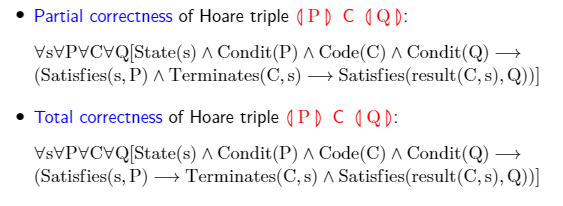
\includegraphics[width=.9\textwidth]{hoare.png}
\end{center}

\tbf{Def} Partial Correctness Proof: Annotated program where each statement has a Hoare triple with justification

\tbf{Def} Logical: After implied rules have been used, ordinary logic proofs must be sued to justify

\tbf{Def} Total Correctness Proof: For each while-loop, identify a strictly-decreasing non-negative integer through the loop (variant)

\tbf{Def} Array Assignment: $\rm A\{i \leftarrow e\}$ is the array with entries given by
$$\rm A\{i \leftarrow e\}[j]  =\begin{cases}\rm e, &\text{if }\rm j=i\\\rm A[j], &\text{if }\rm j\ne i\end{cases}$$

\tbf{Theorem} The Total Correctness Problem is undecidable

\tbf{Theorem} The Partial Correctness Problem is undecidable

\newpage
\tbf{Def} Inference Rules: 
\vspace{-3mm}
\begin{itemize}
    \item Assignment Rule: $Q[E/x]$ is read as $Q$ with $E$ in place of $x$,
    $$\rm \frac{}{\llp Q[E/x] \rrp x = E \llp Q \rrp}$$
    \item Precondition Strengthening: $\emptyset \vdash P \to P'$,
    $$\rm \frac{P \to P', \llp P'\rrp C \llp Q \rrp}{\llp P \rrp C \llp Q \rrp}$$
    \item Postcondition Weakening: $\emptyset \vdash Q' \to Q$,
    $$\rm \frac{\llp P\rrp C \llp Q' \rrp, Q' \to Q}{\llp P \rrp C \llp Q \rrp}$$
    \item Composition: Implicit,
    $$\rm \frac{\llp P\rrp C_1 \llp Q \rrp, \llp Q\rrp C_2 \llp R \rrp}{\llp P \rrp C_1, C_2 \llp R \rrp}$$
    \item If-Then-Else:
    $$\rm \frac{\llp P \wedge B\rrp C_1 \llp Q \rrp, \llp P \wedge \neg B\rrp C_2 \llp Q \rrp}{\llp P \rrp \text{ if } (B), C_1 \text{ else } C_2 \llp Q \rrp}$$
    \item If-Then:
    $$\rm \frac{\llp P \wedge B\rrp C \llp Q \rrp, (P \wedge \neg B) \to Q}{\llp P \rrp \text{ if } (B), C \llp Q \rrp}$$
    \item Partial-While: With loop invariant $\rm I$,
    $$\rm \frac{\llp I \wedge B\rrp C \llp I \rrp}{\llp I \rrp \text{ while } (B), C \llp I \wedge \neg B \rrp}$$
    \item Array-Assignment: With $\rm A\{i \leftarrow e\}[j]  =\begin{cases}\rm e, &\text{if }\rm j=i\\\rm A[j], &\text{if }\rm j\ne i\end{cases}$,
    $$\rm \frac{}{\llp Q[A\{e_1 \leftarrow e_2\}/A] \rrp A[e_1] = e_2 \llp Q \rrp}$$
\end{itemize}


\end{document}